\documentclass[a4paper,12pt]{article}
\usepackage[indonesian]{babel}
\usepackage{graphicx}
\usepackage{multirow}
\usepackage{enumitem}
\usepackage{listings}
\usepackage{wrapfig}
\usepackage[T1]{fontenc}
\usepackage{inconsolata}
\usepackage{lipsum}
\usepackage{adjustbox}


\usepackage{color}
\usepackage[table]{xcolor}
\definecolor{lightgray}{rgb}{0.95, 0.95, 0.95}
\definecolor{darkgray}{rgb}{0.4, 0.4, 0.4}
%\definecolor{purple}{rgb}{0.65, 0.12, 0.82}
\definecolor{editorGray}{rgb}{0.95, 0.95, 0.95}
\definecolor{editorOcher}{rgb}{1, 0.5, 0} % #FF7F00 -> rgb(239, 169, 0)
\definecolor{editorGreen}{rgb}{0, 0.5, 0} % #007C00 -> rgb(0, 124, 0)
\definecolor{orange}{rgb}{1,0.45,0.13}		
\definecolor{olive}{rgb}{0.17,0.59,0.20}
\definecolor{brown}{rgb}{0.69,0.31,0.31}
\definecolor{purple}{rgb}{0.38,0.18,0.81}
\definecolor{lightblue}{rgb}{0.1,0.57,0.7}
\definecolor{lightred}{rgb}{1,0.4,0.5}
\usepackage{upquote}
\usepackage{listings}
% CSS
\lstdefinelanguage{CSS}{
  keywords={color,background-image:,margin,padding,font,weight,display,position,top,left,right,bottom,list,style,border,size,white,space,min,width, transition:, transform:, transition-property, transition-duration, transition-timing-function},	
  sensitive=true,
  morecomment=[l]{//},
  morecomment=[s]{/*}{*/},
  morestring=[b]',
  morestring=[b]",
  alsoletter={:},
  alsodigit={-}
}

% JavaScript
\lstdefinelanguage{JavaScript}{
  morekeywords={typeof, new, true, false, catch, function, return, null, catch, switch, var, if, in, while, do, else, case, break},
  morecomment=[s]{/*}{*/},
  morecomment=[l]//,
  morestring=[b]",
  morestring=[b]'
}

\lstdefinelanguage{HTML5}{
  language=html,
  sensitive=true,	
  alsoletter={<>=-},	
  morecomment=[s]{<!-}{-->},
  tag=[s],
  otherkeywords={
  % General
  >,
  % Standard tags
	<!DOCTYPE,
  </html, <html, <head, <title, </title, <style, </style, <link, </head, <meta, />,
	% body
	</body, <body,
	% Divs
	</div, <div, </div>, 
	% Paragraphs
	</p, <p, </p>,
	% scripts
	</script, <script,
  % More tags...
  <canvas, /canvas>, <svg, <rect, <animateTransform, </rect>, </svg>, <video, <source, <iframe, </iframe>, </video>, <image, </image>, <header, </header, <article, </article
  },
  ndkeywords={
  % General
  =,
  % HTML attributes
  charset=, src=, id=, width=, height=, style=, type=, rel=, href=,
  % SVG attributes
  fill=, attributeName=, begin=, dur=, from=, to=, poster=, controls=, x=, y=, repeatCount=, xlink:href=,
  % properties
  margin:, padding:, background-image:, border:, top:, left:, position:, width:, height:, margin-top:, margin-bottom:, font-size:, line-height:,
	% CSS3 properties
  transform:, -moz-transform:, -webkit-transform:,
  animation:, -webkit-animation:,
  transition:,  transition-duration:, transition-property:, transition-timing-function:,
  }
}

\lstdefinestyle{htmlcssjs} {%
  % General design
%  backgroundcolor=\color{editorGray},
  basicstyle={\footnotesize\ttfamily},   
  frame=b,
  % line-numbers
  xleftmargin={0.75cm},
  numbers=left,
  stepnumber=1,
  firstnumber=1,
  numberfirstline=true,	
  % Code design
  identifierstyle=\color{black},
  keywordstyle=\color{blue}\bfseries,
  ndkeywordstyle=\color{editorGreen}\bfseries,
  stringstyle=\color{editorOcher}\ttfamily,
  commentstyle=\color{brown}\ttfamily,
  % Code
  language=HTML5,
  alsolanguage=JavaScript,
  alsodigit={.:;},	
  tabsize=2,
  showtabs=false,
  showspaces=false,
  showstringspaces=false,
  extendedchars=true,
  breaklines=true,
}
\lstset{
    frame=single,
    language=htmlcssjs,
}
%

\graphicspath{ {./img/} }
\begin{document}
\title{ {\Large Laporan Praktikum}\\ Pemrograman Web Client\\{\Large Pertemuan 2}}

\author{Aldzikri Dwijayanto Prathama 
	\\195410189
	\\Informatika}
\makeatletter
\begin{titlepage}
	\begin{center}
		{\huge \bfseries \@title }\\[14ex]
		
\includegraphics[scale=.8]{logo}\\[4ex]
		{\large \@author}\\[12ex]
		{\large \bfseries {SEKOLAH TINGGI MANAJEMEN INFORMATIKA DAN KOMPUTER
				AKAKOM YOGYAKARTA}}
	\end{center}


%{\large \@date} 
\end{titlepage}
\makeatother
%\maketitle
\newpage
\tableofcontents
\newpage
\section{Tujuan}
\begin{enumerate}
    \item Menuliskan script HTML sesuai struktur
    \item Menuliskan tag-tag dasar (h1, p, div, span, hr, br)
    \item Menuliskan script hyperlink
    \item Menuliskan script list (ul dan ol)
    \item Menuliskan atribut yang sesuai
\end{enumerate}
\section{Dasar Teori}
HTML (Hyper Text MarkUp Language) adalah standar kode program untuk
pembuatan halaman website, dikembangkan oleh Tim Berners-Lee sekitar tahu 1990.
Kode program HTML menggunakan simbol < > biasa disebut “tag” . Pengetikan kode
html bersifat insensitive case yaitu tidak membedakan huruf besar dengan huruf kecil.
Struktur penulisan html adalah sebagai berikut:
\begin{lstlisting}[language=HTML5]
<!DOCTYPE html>
<html>
<head>
</head>
<body>
</body>
</html>
\end{lstlisting}

\newpage

\section{Pembahasan}
\subsection{Praktik}
\subsubsection{Praktik 1}
\begin{lstlisting}
<!DOCTYPE html>
<html>
    <head>
        <title>Page Title</title>
    </head>
    <body>
        <h1> DAFTAR MATA KULIAH JENJANG D3 & S1 </h1>
        <hr>
        <h3> Pilih Semester </h3>
        Semester Ganjil
        Semester Genap
    </body>
</html>
\end{lstlisting}
Dokumen html tersebut memiliki beberapa tag, diantaranya tag <h1> yang akan membuat header atau judul, semakin besar angkanya maka akan semakin kecil font yang akan dirender di browser, 
lalu ada tag <hr> yang akan membuat garis. Jika file tersebut dibuka pada browser maka akan seperti berikut:\\
\begin{center}
    
\includegraphics[width=\linewidth]{1.png} 
\end{center}
Agar tulisan "Semester Ganjil" dan "Semester Genap" tidak menjadi satu baris, maka tambahkan tag <br> untuk mengganti baris setelah kalimat "Semester Ganjil".
\begin{lstlisting}
<!DOCTYPE html>
<html>
    <head>
        <title>Page Title</title>
    </head>
    <body>
        <h1> DAFTAR MATA KULIAH JENJANG D3 & S1 </h1>
        <hr>
        <h3> Pilih Semester </h3>
        Semester Ganjil<br>
        Semester Genap
    </body>
</html>
\end{lstlisting}
Sehingga bila file tersebut dibuka kalimat "Semester Ganjil" dan "Semester Genap" akan terpisah seperti berikut:\\
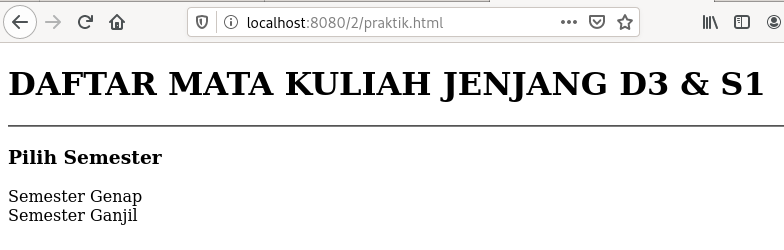
\includegraphics[width=\linewidth]{2.png}

\subsubsection{Praktik 2}
Untuk membuat list tanpa nomor gunakan tag <ul> dan tag <li> untuk point nya.
\begin{lstlisting}
<!DOCTYPE html>
<html>
    <head>
        <title>Praktik</title>
    </head>
    <body>
        <h1> DAFTAR MATA KULIAH JENJANG D3 & S1 </h1>
        <hr>
        <h3> Pilih Semester </h3>
        <ul>
            <li>Semester Genap</li>
            <li>Semester Ganjil</li>
        </ul>
    </body>
</html>
\end{lstlisting}
Maka jika file dibuka di browser maka akan seperti berikut:\\

\includegraphics[width=\linewidth]{3.png}

\subsubsection{Praktik 3}
Sedangkan untuk membuat list bernomor gunakan tag <ol type="1">
\begin{lstlisting}
<!DOCTYPE html>
<html>
    <head>
        <title>Praktik</title>
    </head>
    <body>
        <h1> DAFTAR MATA KULIAH JENJANG D3 & S1 </h1>
        <hr>
        <h3> Pilih Semester </h3>
        <ol type="1">
            <li>Semester Genap</li>
            <li>Semester Ganjil</li>
        </ol>
    </body>
</html>
\end{lstlisting}
Hasilnya seperti berikut:\\
\begin{center}
    
\includegraphics[width=\linewidth]{4.png}
\end{center}
Untuk penomoran dengan tipe lain bisa dideklarasikan dengan type, untuk penomoran dengan angka romawi maka akan seperti berikut:
\begin{lstlisting}
<!DOCTYPE html>
<html>
    <head>
        <title>Praktik</title>
    </head>
    <body>
        <h1> DAFTAR MATA KULIAH JENJANG D3 & S1 </h1>
        <hr>
        <h3> Pilih Semester </h3>
        <ol type="I">
            <li>Semester Genap</li>
            <li>Semester Ganjil</li>
        </ol>
    </body>
</html>
\end{lstlisting}
\begin{center}
    
\includegraphics[width=\linewidth]{1a.png}
\end{center}

\subsubsection{Praktik 4}
Untuk membuat list gabungan bisa dengan mendeklarasikan kembali environment list setelah tag <li>
\begin{lstlisting}
<!DOCTYPE html>
<html>
    <head>
        <title>Praktik</title>
    </head>
    <body>
        <h1> DAFTAR MATA KULIAH JENJANG D3 & S1 </h1>
        <hr>
        <h3> Pilih Semester </h3>
        <ol type="1">
            <li>Semester Genap</li>
            <ul>
                <li>2016/2017</li>
                <li>2018/2019</li>
            </ul>
            <li>Semester Ganjil</li>
            <ul>
                <li>2016/2017</li>
                <li>2018/2019</li>
            </ul>
        </ol>
    </body>
</html>
\end{lstlisting}
Hasilnya seperti berikut:\\
\begin{center}
    
\includegraphics[width=\linewidth]{5.png}
\end{center}

\subsubsection{Praktik 5}
Untuk mencamtumkan link yang mengarah ke file yang masih berada di lokasi yang sama gunakan tag <a href="namafile"> Deskripsi </a>
\begin{lstlisting}
<!DOCTYPE html>
<html>
    <body>
        <h2>HTML Local Links</h2>
        <a href="gabungan.html"> Pilihan Semester </a>
    </body>
</html>
\end{lstlisting}
Maka akan tercipta link ketika file dibuka di browser
\begin{center}
    
\includegraphics[width=\linewidth]{6.png}
\end{center}

Sedangkan untuk mencantumkan link yang mengarah ke website lain, tulis url-nya ke dalam tag
\begin{lstlisting}
<!DOCTYPE html>
<html>
    <body>
        <h2>HTML Links</h2>
        <a href="https://www.akakom.ac.id"> Kunjungi Kampus Kami </a>
    </body>
</html>
\end{lstlisting}
Hasilnya seperti berikut:
\begin{center}
    
\includegraphics[width=\linewidth]{7.png}
\end{center}

\subsection{Latihan}
\begin{lstlisting}
<!DOCTYPE html>
<html>
    <head>
        <title>Praktik</title>
    </head>
    <body>
        <h3> DAFTAR MENU </h3>
        <ol type="A">
            <li>Makanan</li>
            <ol type="1">
                <li>Bakso</li>
                <li>Mie Ayam</li>
                <li>Soto</li>
            </ol>
            <li>Minuman</li>
            <ol type="1">
                <li>Es Teh</li>
                <li>Es Jeruk</li>
                <li>Air Mineral</li>
            </ol>
        </ol>
    </body>
</html>
\end{lstlisting}
Untuk membuat menu, gunakan list gabungan seperti pada Praktik 4, tetapi type diganti menjadi "A" sehingga penomorannya menggunakan alfabet, sedangkan list didalmnya menggunkan 
type "1" sehingga penomorannya menggunakan angka
\begin{center}
    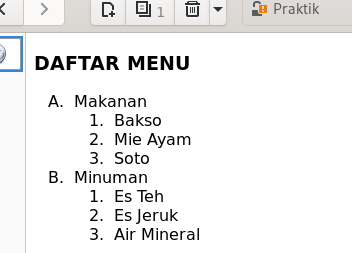
\includegraphics[width=\linewidth]{8.png}
\end{center}

\section{Kesimpulan}
\end{document}
